\documentclass[aspectratio=169,11pt]{beamer}
\usepackage[utf8]{inputenc}
\usepackage[T1]{fontenc}
\usepackage[spanish]{babel}
\usepackage{amsmath,amssymb}
\usepackage{tikz}
\usetikzlibrary{arrows.meta,angles,calc,positioning}
\usetheme{Madrid}
\usecolortheme{default}
\setbeamertemplate{navigation symbols}{}
\setbeamertemplate{blocks}[rounded][shadow=false]
\newcommand{\ang}[1]{\angle #1^\circ}

\title[QFT y no linealidades]{Paso 15: QFT y sistemas no lineales}
\subtitle{Convertir la no linealidad en una familia que ya sabemos tratar}
\author{Curso de control robusto (QFT)}
\date{}
\begin{document}
\begin{frame}\titlepage\end{frame}

\begin{frame}{Dónde encaja este paso}
  \tiny
  \begin{enumerate}\setlength{\itemsep}{-2pt}
    \item[1.] Números complejos \hfill \textcolor{gray}{(hecho)}
    \item[2.] Funciones de transferencia: $s$, polos y ceros \hfill \textcolor{gray}{(hecho)}
    \item[3.] Respuesta en frecuencia: $s=j\omega$, magnitud y fase \hfill \textcolor{gray}{(hecho)}
    \item[4.] Decibelios y escala logarítmica (Bode) \hfill \textcolor{gray}{(hecho)}
    \item[5.] Realimentación: $L$, $T=\frac{L}{1+L}$, $S=\frac{1}{1+L}$ \hfill \textcolor{gray}{(hecho)}
    \item[6.] Nichols chart \hfill \textcolor{gray}{(hecho)}
    \item[7.] Incertidumbre y templates \hfill \textcolor{gray}{(hecho)}
    \item[8.] Especificaciones $\rightarrow$ bounds \hfill \textcolor{gray}{(hecho)}
    \item[9.] Loop shaping, prefiltro y verificación \hfill \textcolor{gray}{(hecho)}
    \item[10.] QFT en control digital \hfill \textcolor{gray}{(hecho)}
    \item[11.] Dos caminos digitales: $z$ y $w$ \hfill \textcolor{gray}{(hecho)}
    \item[12.] Estabilidad, límites, más especificaciones y caso real \hfill \textcolor{gray}{(hecho)}
    \item[13.] Muestreo por eventos con periodo base $T$ \hfill \textcolor{gray}{(hecho)}
    \item[14.] Sistemas de dos estados: lazo interno y externo \hfill \textcolor{gray}{(hecho)}
    \item[\textbf{15.}] \textbf{QFT y sistemas no lineales} \hfill $\leftarrow$ estamos aquí
    \item[16.] Algoritmos de QFT: cómo funcionan por dentro
    \item[17.] QFT en Python: una biblioteca paso a paso
    \item[18.] QFT en MATLAB: el mismo código, otra sintaxis
    \item[19.] Historia, panorama y bibliografía
  \end{enumerate}
  \vspace{2pt}
  \begin{block}{Objetivo de hoy}
    QFT trabaja con respuestas en frecuencia de plantas \textbf{lineales}. Los sistemas reales tienen saturación, fricción, zona muerta, amortiguamiento no lineal. La idea de Horowitz: sustituir la no linealidad por un \textbf{conjunto de plantas lineales} que la envuelve, y diseñar para todo el conjunto.
  \end{block}
\end{frame}

\begin{frame}{La idea: una no linealidad es otra forma de incertidumbre}
  \small
  \begin{columns}[T]
  \begin{column}{0.52\textwidth}
    \begin{itemize}
      \item Una planta no lineal responde distinto según la \textbf{amplitud} de las señales.
      \item Si acotamos esas amplitudes (por la referencia, la perturbación, los límites físicos), la no linealidad se comporta como un \textbf{parámetro incierto}.
      \item Ese parámetro cae en un intervalo: ya sabemos hacer templates (paso 7), bounds (8) y loop shaping (9).
    \end{itemize}
  \end{column}
  \begin{column}{0.44\textwidth}
    \begin{block}{Tres traducciones}
      \footnotesize
      \begin{tabular}{l|l}
        No linealidad & Equivale a\\\hline
        Amortiguamiento & sector, $a\in[a_1,a_2]$\\
        Saturación & ganancia $K$ más baja\\
        Fricción de Coulomb & perturbación acotada
      \end{tabular}
    \end{block}
  \end{column}
  \end{columns}
  \vspace{3pt}
  \begin{alertblock}{Con una condición}
    La equivalencia vale \textbf{mientras las amplitudes estén dentro de lo supuesto}. Fuera, no hay garantía: por eso al final siempre se simula el lazo no lineal.
  \end{alertblock}
\end{frame}

\begin{frame}{Ejemplo 1: amortiguamiento no lineal $\Rightarrow$ sector}
  \small
  Planta: $\dot x_1=x_2$, $\dot x_2=-\varphi(x_2)+K\,u$, con $\varphi(v)=v+0.5\,v^3$ y $K\in[1,5]$.
  \begin{itemize}
    \item Para $|v|\le2$: $\;1\cdot v\le\varphi(v)\le3\cdot v$ (para $v>0$). Es un \textbf{sector} $[1,3]$.
    \item Una planta con $\dot x_2=-a\,x_2+Ku$ y $a\in[1,3]$ es \textbf{exactamente nuestra familia} de siempre.
  \end{itemize}
  \begin{block}{Consecuencia}
    El diseño del paso 9, $G=5\,\frac{1+s/2}{1+s/20}$ con $F=\frac{1.2}{s+1.2}$, \textbf{sirve sin cambios} mientras la velocidad cumpla $|x_2|\le2$.
  \end{block}
  \begin{itemize}
    \item El sector es una cota \textbf{conservadora}: la nueva planta puede ir más rápida que la familia en algunos instantes, pero nunca fuera del sector.
    \item Con $|x_2|\le v_{max}$ el sector es $[1,\,1+0.5\,v_{max}^2]$.
  \end{itemize}
\end{frame}

\begin{frame}{Simulación con la planta no lineal}
  \footnotesize
  \centering
  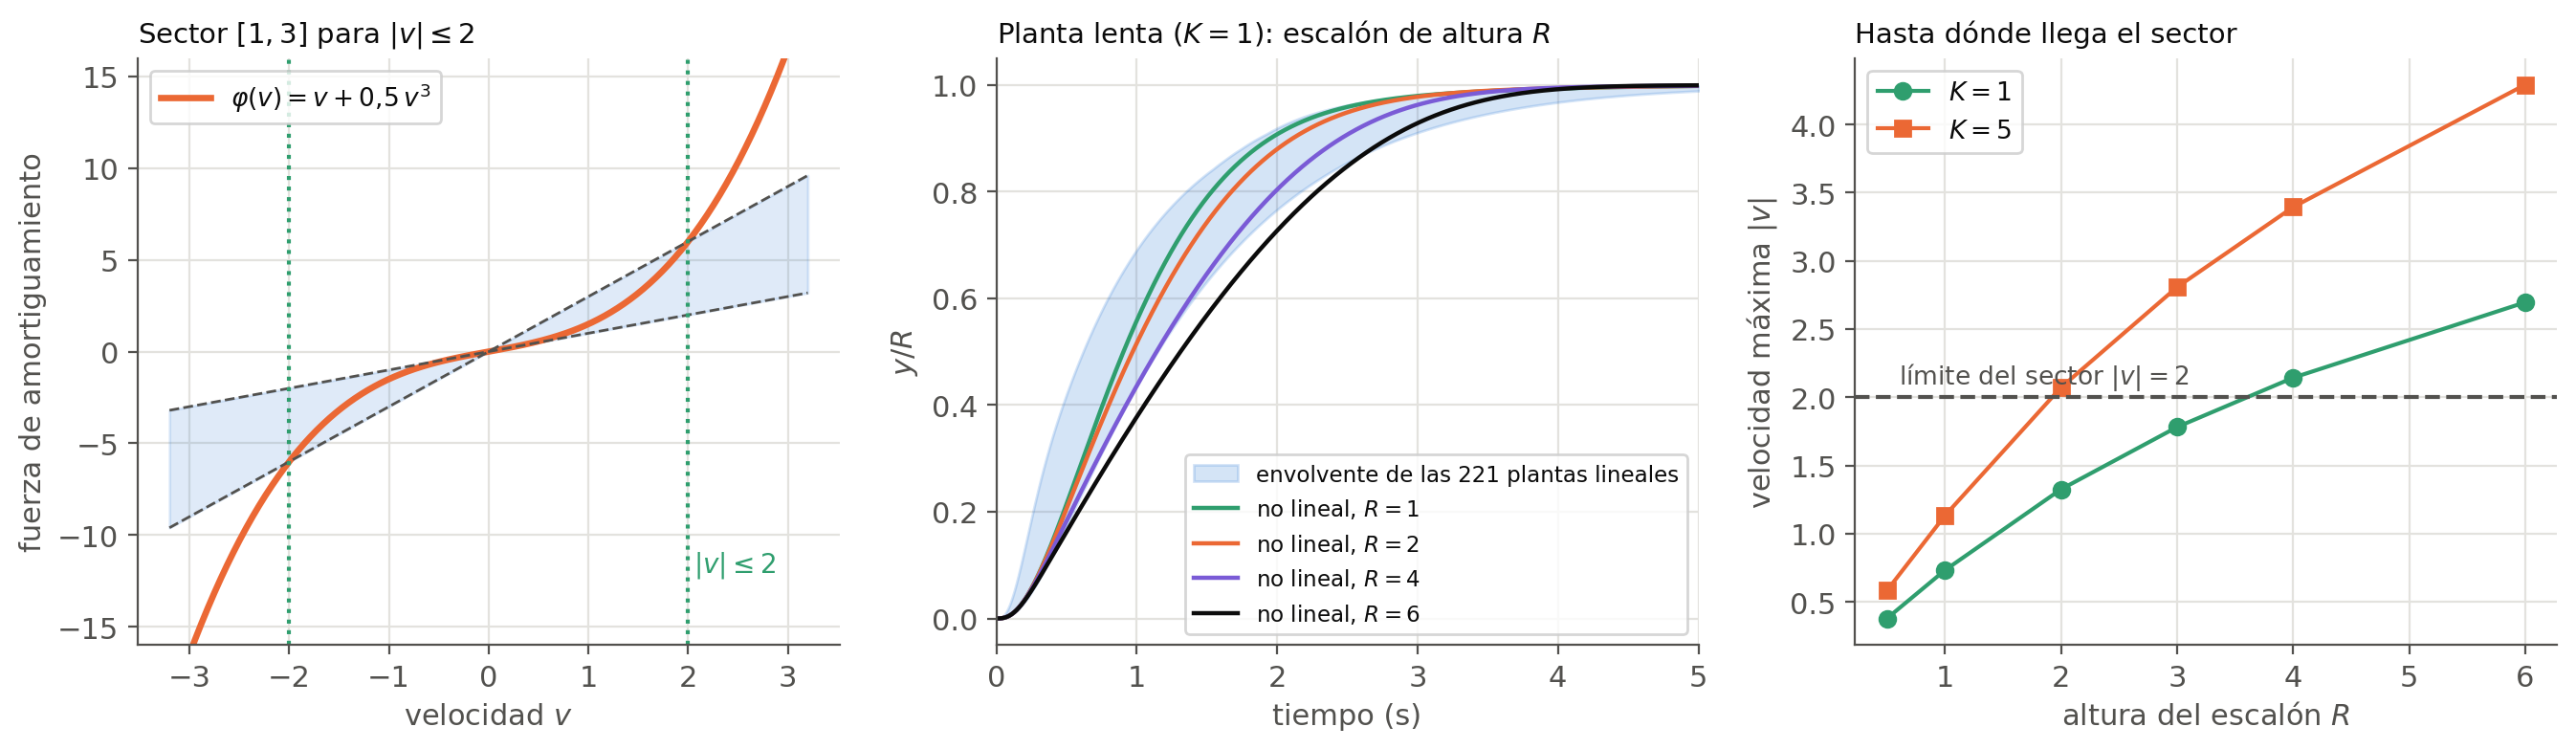
\includegraphics[width=\textwidth]{fig/amortiguamiento.png}\\[2pt]
  \begin{itemize}
    \item Centro: la banda azul es la envolvente de las 221 respuestas lineales (escalón de altura 1). Las respuestas no lineales, normalizadas por la altura $R$, quedan dentro (a lo sumo $0.002$ fuera) hasta $R=4$.
    \item Con $R=6$ la planta lenta ($K=1$) se sale \textbf{por abajo} de la envolvente en $0.066$ (la envolvente mide hasta $0.27$ de ancho).
    \item Derecha: el sector $|v|\le2$ se rebasa con $R\approx2$ ($K=5$) y $R\approx3.7$ ($K=1$). Aun así el lazo aguanta: el sector es \textbf{suficiente}, no necesario.
  \end{itemize}
\end{frame}

\begin{frame}{Resultados numéricos del ejemplo 1}
  \small
  \begin{center}
  \begin{tabular}{c|c|c|c}
    $R$ & $\max|v|$ ($K=1$) & $\max|v|$ ($K=5$) & fuera de la envolvente ($K=1$)\\\hline
    0.5 & 0.38 & 0.58 & $0.0001$\\
    1 & 0.73 & 1.13 & $0.0004$\\
    2 & 1.32 & 2.07 & $0.0012$\\
    4 & 2.14 & 3.39 & $0.0018$\\
    6 & 2.70 & 4.29 & $0.0657$
  \end{tabular}
  \end{center}
  \footnotesize
  Distancia máxima de $y/R$ fuera de la envolvente de la familia lineal, en las 221 plantas, con $F$ y $G$ del paso 9.
  \begin{itemize}
    \item Con $K=3$ y $K=5$, la distancia fue $0.000$ en todos los casos probados.
    \item Lo que importa es la \textbf{velocidad máxima} que alcanza el sistema, que depende de $R$ y de $K$. El diseño del lazo se hace para un \textbf{rango de amplitudes}, no para ``cualquier'' señal.
  \end{itemize}
\end{frame}

\begin{frame}{Ejemplo 2: saturación $\Rightarrow$ ganancia equivalente más baja}
  \small
  \begin{columns}[T]
  \begin{column}{0.5\textwidth}
    Si $u$ supera $u_{max}$, el actuador entrega menos de lo pedido. Para una señal de amplitud $A>u_{max}$ la \textbf{ganancia equivalente} es aproximadamente
    \[ N(A)\approx\frac{u_{max}}{A}. \]
    \begin{itemize}
      \item El rango $\beta\le N\le1$ hace que $K$ se comporte como $K\,N\in[\beta K,\,K]$.
      \item Se añade a la familia: $K_{min}$ baja a $\beta K_{min}$.
      \item Con $K_{min}=1$ y un pico de $u\approx2.6$ ($K=1$, escalón 1), $u_{max}=1$ da $\beta\approx0.4$.
    \end{itemize}
  \end{column}
  \begin{column}{0.46\textwidth}
    \begin{block}{Medido en el diseño del paso 9}
      \footnotesize
      \begin{tabular}{c|c}
        $K_{min}$ & frecuencias que incumplen\\\hline
        1 & 0\\
        0.8 & 11\\
        0.6 & 32\\
        0.5 & 46\\
        0.4 & 159\\
        0.3 & 163
      \end{tabular}
      \\[2pt]
      \scriptsize De 300 frecuencias entre $0.01$ y $60$ rad/s.
    \end{block}
  \end{column}
  \end{columns}
  \vspace{2pt}
  \footnotesize El primer fallo (con $K_{min}=0.8$) es el \textbf{rechazo de perturbación} $|S|\le W_d$, entre $0.44$ y $0.99$ rad/s: menos ganancia, menos rechazo.
\end{frame}

\begin{frame}{La saturación sí importa en la planta lenta}
  \footnotesize
  \centering
  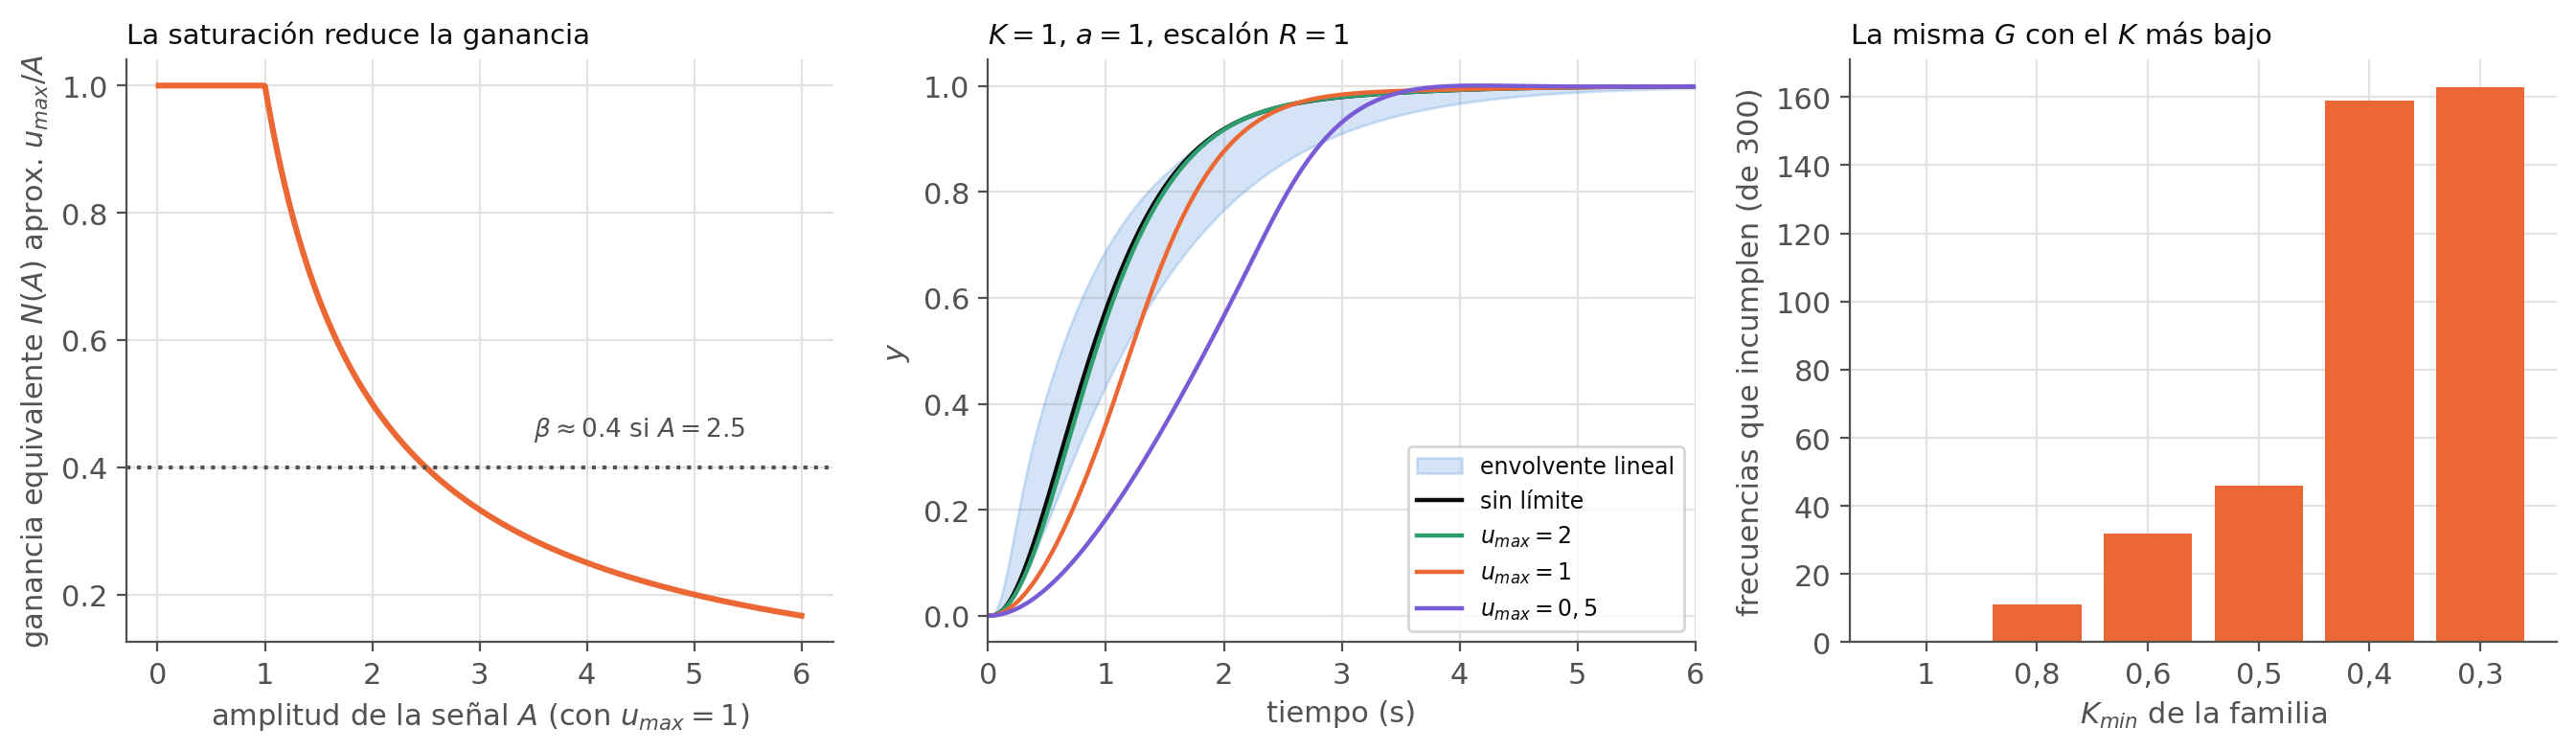
\includegraphics[width=0.93\textwidth]{fig/saturacion.png}\\[0pt]
  \begin{itemize}
    \item Centro: con $u_{max}=1$ la planta $K=1$ tarda claramente más y sale de la envolvente. Con $u_{max}=2$ casi no se nota.
    \item Solo importa el cociente $u_{max}/R$: con escalón $R=2$ y $u_{max}=2$ sale lo mismo que con $R=1$ y $u_{max}=1$ (planta lineal).
    \item Distancia fuera de la envolvente, $R=1$, $K=1$, $a=1$/$a=3$: con $u_{max}=2$: $0.001/0.027$; con $1$: $0.093/0.245$; con $0.5$: $0.277/0.496$. Para $K=5$ es $0.000$ con $u_{max}\ge0.5$.
    \item En el paso 12 casi no importaba porque era $K=5$; con $K=1$ \textbf{sí}.
  \end{itemize}
\end{frame}

\begin{frame}{Ejemplo 3: fricción de Coulomb $\Rightarrow$ perturbación acotada}
  \small
  \begin{columns}[T]
  \begin{column}{0.46\textwidth}
    Fuerza constante $f_c$ que se opone al movimiento: $\dot x_2=-a\,x_2-f_c\,\mathrm{sign}(x_2)+K\,u$.
    \begin{itemize}
      \item No depende de la amplitud de $x_2$: es una \textbf{perturbación de amplitud acotada} $f_c/K$ en la entrada.
      \item El paso 12 ya sabe tratarla: error $\le d/G(0)$.
      \item La planta se detiene cuando $K\,G(0)\,|e|\le f_c$. Con $G(0)=5$:
      \[ |e|\le\frac{f_c}{5\,K}. \]
    \end{itemize}
  \end{column}
  \begin{column}{0.52\textwidth}
    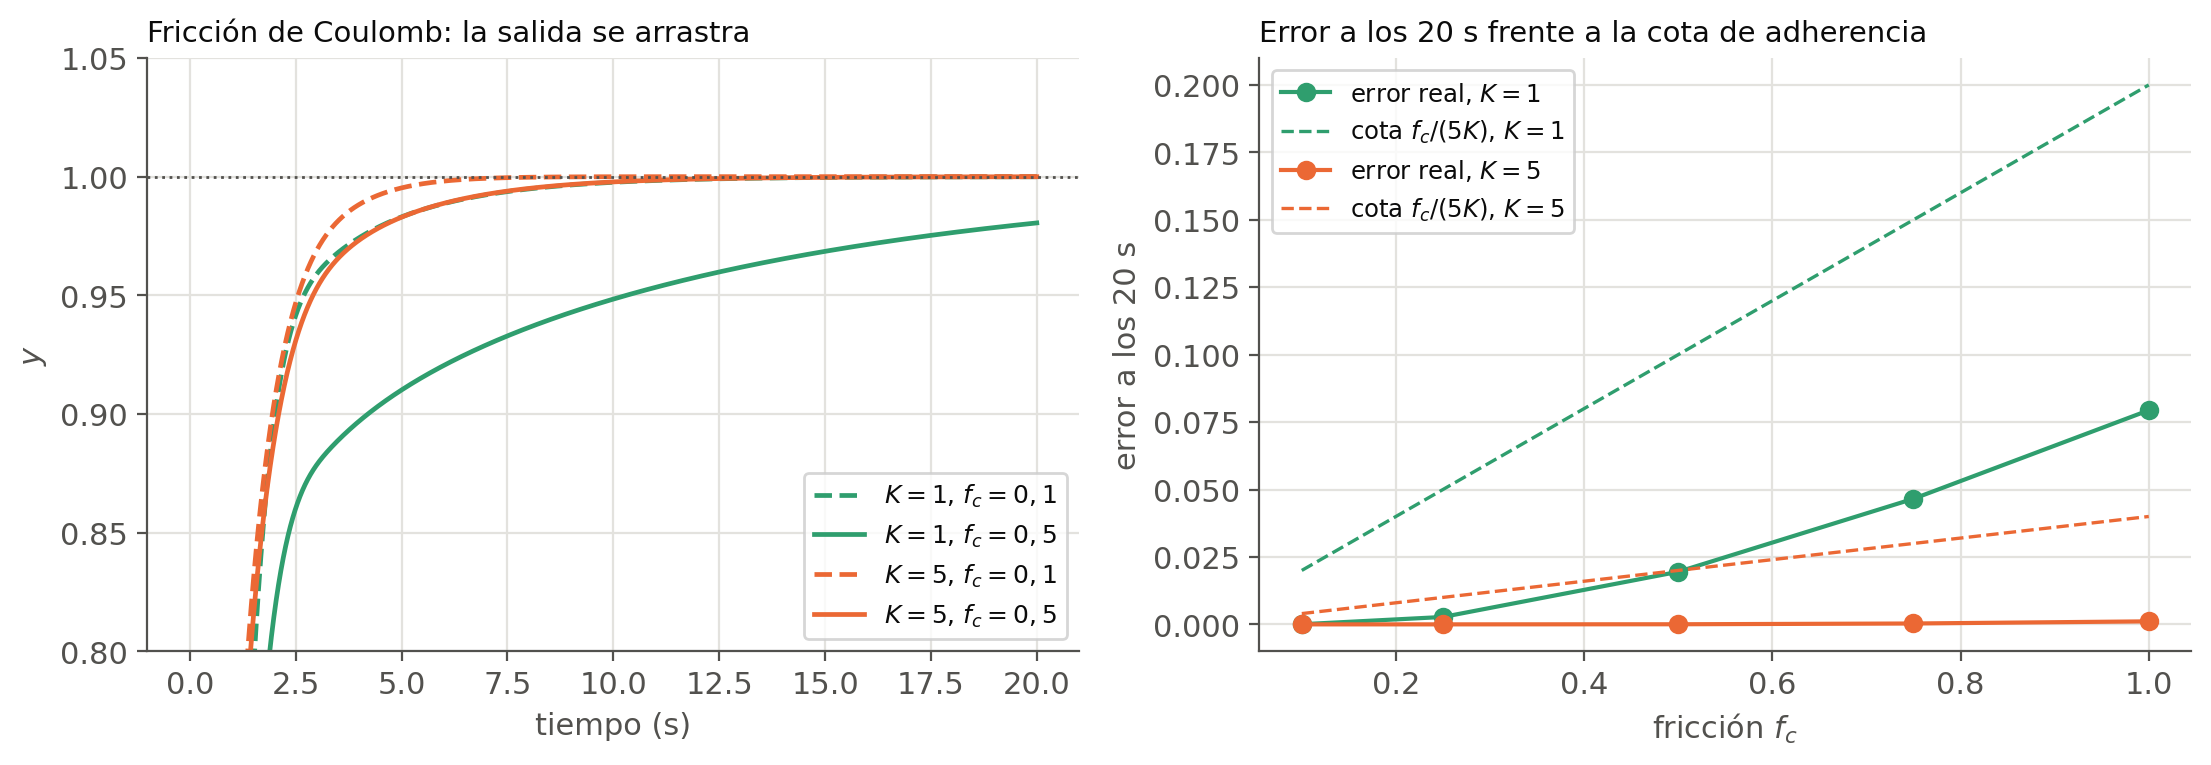
\includegraphics[width=\textwidth]{fig/friccion.png}
  \end{column}
  \end{columns}
  \vspace{2pt}
  \footnotesize
  Simulado con fricción suavizada ($f_c\tanh(v/0.01)$): la salida \textbf{se arrastra} hacia el valor final en vez de pararse. A los 20 s el error vale como mucho $0.08$ ($K=1$, $f_c=1$), siempre por debajo de la cota de adherencia.
\end{frame}

\begin{frame}{Otras no linealidades y la discretización}
  \small
  \begin{itemize}
    \item \textbf{Zona muerta del actuador} (un motor que no se mueve con $|u|<d$): es una perturbación acotada $\le d$ más una pérdida de ganancia para señales pequeñas. Se trata con la misma receta que la fricción.
    \item \textbf{Cuantización del sensor} (paso $q$): error de medida $|e|\le q/2$, igual que el umbral del paso 13. La desviación de $y$ queda por debajo de $\|t\|_1\,q/2$ con $\|t\|_1=1.42$.
  \end{itemize}
  \begin{center}
  \footnotesize
  \begin{tabular}{c|c|c}
    $q$ & desviación de $y$ medida & cota $1.42\,q/2$\\\hline
    0.01 & 0.0055 & 0.0071\\
    0.05 & 0.0258 & 0.0356\\
    0.10 & 0.0492 & 0.0712
  \end{tabular}
  \end{center}
  \footnotesize
  (Diseño del paso 12 a $T_s=0.04$; cuatro esquinas; escalón de $1$.)
  \begin{itemize}
    \item \textbf{Saturación en discreto}: guardar el $u$ \textbf{saturado} en la ecuación en diferencias (paso 12), no el calculado.
  \end{itemize}
\end{frame}

\begin{frame}{Estabilidad con no linealidades}
  \small
  \begin{itemize}
    \item Los criterios de \textbf{estabilidad absoluta} (círculo, Popov) usan el mismo concepto de sector: la no linealidad $\varphi$ está en $[k_1,k_2]$ y se exige que $L(j\omega)$ evite una región.
    \item Dan estabilidad \textbf{garantizada} para toda no linealidad dentro del sector, pero son \textbf{conservadores}: pueden pedir más margen del necesario.
    \item QFT permite cubrir lo mismo desde el diseño, con bounds sobre el lazo, y a la vez especificar prestaciones.
  \end{itemize}
  \begin{alertblock}{Lo que ni el sector ni QFT garantizan}
    Los \textbf{ciclos límite}, el \textbf{stick-slip} (con fricción estática y acción integral, el sistema oscila parándose y arrancando) y la dependencia de la \textbf{condición inicial}. Los dos primeros se buscan con simulación o con función descriptiva.
  \end{alertblock}
  En el ejemplo, $G(0)=5$ no tiene integrador: no hay \textbf{hunting}. Si se añade acción integral, hay que simular con fricción estática.
\end{frame}

\begin{frame}{Procedimiento}
  \small
  \begin{enumerate}
    \item \textbf{Acotar las señales}: amplitud de la referencia, de la perturbación, del mando.
    \item \textbf{Traducir} cada no linealidad: sector $\to$ parámetro; saturación $\to$ ganancia; fricción o zona muerta $\to$ perturbación; cuantización $\to$ ruido acotado.
    \item \textbf{Ampliar la familia} y repetir los pasos 7 a 9 (bounds, loop shaping, prefiltro).
    \item \textbf{Verificar} con la planta no lineal real, en simulación, para los extremos de amplitud y de parámetros.
    \item Si la verificación falla en una esquina: reducir las amplitudes (limitar la referencia o su velocidad) o ampliar la familia.
  \end{enumerate}
  \begin{block}{Lo que cuesta}
    La familia se hace más grande, y el diseño más exigente: por ejemplo, $K_{min}=0.5$ en lugar de $1$ obliga a rediseñar $G$ (46 frecuencias incumplen con el diseño actual).
  \end{block}
\end{frame}

\begin{frame}{Las dos técnicas de Horowitz para no linealidades}
  \small
  QFT trata las plantas no lineales (NL) o variables en el tiempo reduciéndolas \textbf{rigurosamente} a un conjunto de problemas lineales invariantes (LTI):
  \begin{enumerate}
    \item \textbf{Conjunto LTI equivalente} (Horowitz, 1976, 1981a): para un conjunto de entradas y salidas deseadas, se busca un conjunto de plantas LTI que dé las mismas salidas. Caro de calcular; una mejora (Horowitz, 1981b) cancela la parte no lineal de la planta nominal.
    \item \textbf{No linealidad como perturbación equivalente} (Horowitz, 1982c): el control se diseña para la parte lineal, con una especificación de rechazo de la perturbación equivalente.
  \end{enumerate}
  \begin{itemize}
    \item Saturación: Horowitz (1983) y Horowitz y Liao (1986b). Backlash: Oldak y otros (1994). Estabilidad: Baños y Barreiro (2000).
    \item Lo que hicimos en este paso (sector, saturación $\beta=u_{\max}/A$, fricción de Coulomb) es la \textbf{segunda} técnica en su versión más simple.
  \end{itemize}
\end{frame}

\begin{frame}{Resumen}
  \small
  \begin{itemize}
    \item Una no linealidad con amplitudes acotadas es una \textbf{familia de plantas lineales}: sector, ganancia equivalente, perturbación o ruido acotados.
    \item Ejemplo 1: $\varphi(v)=v+0.5v^3$ con $|v|\le2$ es exactamente $a\in[1,3]$; el diseño del paso 9 sirve sin cambios hasta $R=4$.
    \item Ejemplo 2: la saturación baja $K_{min}$; con $K_{min}=0.8$ ya fallan $11$ frecuencias.
    \item Ejemplo 3: la fricción da un error estacionario acotado por $f_c/(G(0)K)$.
    \item QFT no ve ciclos límite ni stick-slip: simular siempre.
  \end{itemize}
  \begin{block}{Ejercicio}
    (1) Con $u_{max}=1$ y una señal de amplitud $A=2.5$, ¿cuánto vale $\beta$? (2) Con $K=2$, $f_c=0.3$ y $G(0)=5$, ¿cuál es la cota de error? (3) Con un sensor de cuantización $q=0.02$, ¿cuál es la cota de desviación de $y$?
  \end{block}
\end{frame}

\appendix
\begin{frame}{Solución del ejercicio}
  \footnotesize
  \textbf{1.} $\beta=u_{max}/A=1/2.5=0.4$.\\[3pt]
  \textbf{2.} $|e|\le f_c/(G(0)K)=0.3/(5\cdot2)=0.03$.\\[3pt]
  \textbf{3.} $\|t\|_1\,q/2=1.42\cdot0.01=0.0142$ (con el diseño del paso 12; la desviación medida a $q=0.01$ fue $0.0055$, así que la cota es conservadora).
\end{frame}
\end{document}
